\PassOptionsToPackage{unicode=true}{hyperref} % options for packages loaded elsewhere
\PassOptionsToPackage{hyphens}{url}
%
\documentclass[]{article}
\usepackage{lmodern}
\usepackage{amssymb,amsmath}
\usepackage{ifxetex,ifluatex}
\usepackage{fixltx2e} % provides \textsubscript
\ifnum 0\ifxetex 1\fi\ifluatex 1\fi=0 % if pdftex
  \usepackage[T1]{fontenc}
  \usepackage[utf8]{inputenc}
  \usepackage{textcomp} % provides euro and other symbols
\else % if luatex or xelatex
  \usepackage{unicode-math}
  \defaultfontfeatures{Ligatures=TeX,Scale=MatchLowercase}
\fi
% use upquote if available, for straight quotes in verbatim environments
\IfFileExists{upquote.sty}{\usepackage{upquote}}{}
% use microtype if available
\IfFileExists{microtype.sty}{%
\usepackage[]{microtype}
\UseMicrotypeSet[protrusion]{basicmath} % disable protrusion for tt fonts
}{}
\IfFileExists{parskip.sty}{%
\usepackage{parskip}
}{% else
\setlength{\parindent}{0pt}
\setlength{\parskip}{6pt plus 2pt minus 1pt}
}
\usepackage{hyperref}
\hypersetup{
            pdftitle={Programming Approaches for Bioinformatics Exam},
            pdfauthor={Maiolino Aurelio - 923271},
            pdfborder={0 0 0},
            breaklinks=true}
\urlstyle{same}  % don't use monospace font for urls
\usepackage[margin=1in]{geometry}
\usepackage{color}
\usepackage{fancyvrb}
\newcommand{\VerbBar}{|}
\newcommand{\VERB}{\Verb[commandchars=\\\{\}]}
\DefineVerbatimEnvironment{Highlighting}{Verbatim}{commandchars=\\\{\}}
% Add ',fontsize=\small' for more characters per line
\usepackage{framed}
\definecolor{shadecolor}{RGB}{248,248,248}
\newenvironment{Shaded}{\begin{snugshade}}{\end{snugshade}}
\newcommand{\AlertTok}[1]{\textcolor[rgb]{0.94,0.16,0.16}{#1}}
\newcommand{\AnnotationTok}[1]{\textcolor[rgb]{0.56,0.35,0.01}{\textbf{\textit{#1}}}}
\newcommand{\AttributeTok}[1]{\textcolor[rgb]{0.77,0.63,0.00}{#1}}
\newcommand{\BaseNTok}[1]{\textcolor[rgb]{0.00,0.00,0.81}{#1}}
\newcommand{\BuiltInTok}[1]{#1}
\newcommand{\CharTok}[1]{\textcolor[rgb]{0.31,0.60,0.02}{#1}}
\newcommand{\CommentTok}[1]{\textcolor[rgb]{0.56,0.35,0.01}{\textit{#1}}}
\newcommand{\CommentVarTok}[1]{\textcolor[rgb]{0.56,0.35,0.01}{\textbf{\textit{#1}}}}
\newcommand{\ConstantTok}[1]{\textcolor[rgb]{0.00,0.00,0.00}{#1}}
\newcommand{\ControlFlowTok}[1]{\textcolor[rgb]{0.13,0.29,0.53}{\textbf{#1}}}
\newcommand{\DataTypeTok}[1]{\textcolor[rgb]{0.13,0.29,0.53}{#1}}
\newcommand{\DecValTok}[1]{\textcolor[rgb]{0.00,0.00,0.81}{#1}}
\newcommand{\DocumentationTok}[1]{\textcolor[rgb]{0.56,0.35,0.01}{\textbf{\textit{#1}}}}
\newcommand{\ErrorTok}[1]{\textcolor[rgb]{0.64,0.00,0.00}{\textbf{#1}}}
\newcommand{\ExtensionTok}[1]{#1}
\newcommand{\FloatTok}[1]{\textcolor[rgb]{0.00,0.00,0.81}{#1}}
\newcommand{\FunctionTok}[1]{\textcolor[rgb]{0.00,0.00,0.00}{#1}}
\newcommand{\ImportTok}[1]{#1}
\newcommand{\InformationTok}[1]{\textcolor[rgb]{0.56,0.35,0.01}{\textbf{\textit{#1}}}}
\newcommand{\KeywordTok}[1]{\textcolor[rgb]{0.13,0.29,0.53}{\textbf{#1}}}
\newcommand{\NormalTok}[1]{#1}
\newcommand{\OperatorTok}[1]{\textcolor[rgb]{0.81,0.36,0.00}{\textbf{#1}}}
\newcommand{\OtherTok}[1]{\textcolor[rgb]{0.56,0.35,0.01}{#1}}
\newcommand{\PreprocessorTok}[1]{\textcolor[rgb]{0.56,0.35,0.01}{\textit{#1}}}
\newcommand{\RegionMarkerTok}[1]{#1}
\newcommand{\SpecialCharTok}[1]{\textcolor[rgb]{0.00,0.00,0.00}{#1}}
\newcommand{\SpecialStringTok}[1]{\textcolor[rgb]{0.31,0.60,0.02}{#1}}
\newcommand{\StringTok}[1]{\textcolor[rgb]{0.31,0.60,0.02}{#1}}
\newcommand{\VariableTok}[1]{\textcolor[rgb]{0.00,0.00,0.00}{#1}}
\newcommand{\VerbatimStringTok}[1]{\textcolor[rgb]{0.31,0.60,0.02}{#1}}
\newcommand{\WarningTok}[1]{\textcolor[rgb]{0.56,0.35,0.01}{\textbf{\textit{#1}}}}
\usepackage{graphicx,grffile}
\makeatletter
\def\maxwidth{\ifdim\Gin@nat@width>\linewidth\linewidth\else\Gin@nat@width\fi}
\def\maxheight{\ifdim\Gin@nat@height>\textheight\textheight\else\Gin@nat@height\fi}
\makeatother
% Scale images if necessary, so that they will not overflow the page
% margins by default, and it is still possible to overwrite the defaults
% using explicit options in \includegraphics[width, height, ...]{}
\setkeys{Gin}{width=\maxwidth,height=\maxheight,keepaspectratio}
\setlength{\emergencystretch}{3em}  % prevent overfull lines
\providecommand{\tightlist}{%
  \setlength{\itemsep}{0pt}\setlength{\parskip}{0pt}}
\setcounter{secnumdepth}{0}
% Redefines (sub)paragraphs to behave more like sections
\ifx\paragraph\undefined\else
\let\oldparagraph\paragraph
\renewcommand{\paragraph}[1]{\oldparagraph{#1}\mbox{}}
\fi
\ifx\subparagraph\undefined\else
\let\oldsubparagraph\subparagraph
\renewcommand{\subparagraph}[1]{\oldsubparagraph{#1}\mbox{}}
\fi

% set default figure placement to htbp
\makeatletter
\def\fps@figure{htbp}
\makeatother

\usepackage{fvextra}
\DefineVerbatimEnvironment{Highlighting}{Verbatim}{breaklines,breakanywhere=true,commandchars=\\\{\}}
\fvset{breaklines=true, breakanywhere=true}
\renewcommand{\contentsname}{Index}

\title{Programming Approaches for Bioinformatics Exam}
\author{Maiolino Aurelio - 923271}
\date{27-06-2025}

\begin{document}
\maketitle

{
\setcounter{tocdepth}{2}
\tableofcontents
}
\thispagestyle{empty}

\newpage
\pagenumbering{arabic}
\setcounter{page}{1}

\hypertarget{introduction-rileggi-attentamente-potrebbero-esserci-dei-cazzi}{%
\section{Introduction: Rileggi attentamente, potrebbero esserci dei
CAZZI}\label{introduction-rileggi-attentamente-potrebbero-esserci-dei-cazzi}}

The repository for this exam can be found on my
\href{https://github.com/Maiolino-Au/ProgrAppBioinfo_Exam}{GitHub}

controlla i link, che forse cambi i nomi delle cartelle

rimuovi gli eval=FALSE

\newpage

\hypertarget{part-1-docker}{%
\section{Part 1: Docker}\label{part-1-docker}}

Docker is this

The Dockerfile is that and can be found
\href{https://github.com/Maiolino-Au/ProgrAppBioinfo_Exam/blob/main/Docker_container}{here}

\hypertarget{building-the-docker-the-dockerfile}{%
\subsection{Building the Docker: the
Dockerfile}\label{building-the-docker-the-dockerfile}}

Build a container from a base Ubuntu image, v20.04 was chosen due to its
proven stability.

\begin{Shaded}
\begin{Highlighting}[]
\KeywordTok{FROM}\NormalTok{ ubuntu:20.04}

\KeywordTok{ENV}\NormalTok{ DEBIAN_FRONTEND=noninteractive}

\KeywordTok{LABEL}\NormalTok{ maintainer=}\StringTok{"aurelio.maiolino@edu.unito.it"}
\end{Highlighting}
\end{Shaded}

The base Ubuntu image is just that, an Ubuntu installation with not a
lot more inside it. It is therefore necessary to install various
packages.

Some notable are

\begin{itemize}
\tightlist
\item
  curl:
\item
  b
\end{itemize}

ne mancano ancora

\begin{Shaded}
\begin{Highlighting}[]
\KeywordTok{RUN}\NormalTok{ apt-get update && apt-get install -y --no-install-recommends \textbackslash{}}
\NormalTok{    software-properties-common \textbackslash{}}
\NormalTok{    dirmngr \textbackslash{}}
\NormalTok{    gpg \textbackslash{}}
\NormalTok{    curl \textbackslash{}}
\NormalTok{    build-essential \textbackslash{}}
\NormalTok{    libcurl4-openssl-dev \textbackslash{}}
\NormalTok{    libssl-dev \textbackslash{}}
\NormalTok{    libxml2-dev \textbackslash{}}
\NormalTok{    libfontconfig1-dev \textbackslash{}}
\NormalTok{    libfreetype6-dev \textbackslash{}}
\NormalTok{    libpng-dev \textbackslash{}}
\NormalTok{    libtiff5-dev \textbackslash{}}
\NormalTok{    libjpeg-dev \textbackslash{}}
\NormalTok{    libharfbuzz-dev \textbackslash{}}
\NormalTok{    libfribidi-dev \textbackslash{}}
\NormalTok{    make \textbackslash{}}
\NormalTok{    cmake \textbackslash{}}
\NormalTok{    gfortran \textbackslash{}}
\NormalTok{    libxt-dev \textbackslash{}}
\NormalTok{    liblapack-dev \textbackslash{}}
\NormalTok{    libblas-dev \textbackslash{}}
\NormalTok{    sudo \textbackslash{}}
\NormalTok{    wget \textbackslash{}}
\NormalTok{    zlib1g-dev \textbackslash{}}
\NormalTok{    libbz2-dev \textbackslash{}}
\NormalTok{    liblzma-dev \textbackslash{}}
\NormalTok{    libncurses5-dev \textbackslash{}}
\NormalTok{    pandoc \textbackslash{}}
\NormalTok{    git}
\end{Highlighting}
\end{Shaded}

After all of this a cleaning step can be useful:

\begin{Shaded}
\begin{Highlighting}[]
\KeywordTok{RUN}\NormalTok{ rm -rf /var/lib/apt/lists/*}
\end{Highlighting}
\end{Shaded}

Add the Cran Repository and install R

\begin{Shaded}
\begin{Highlighting}[]
\CommentTok{# Add the CRAN GPG key and repository for R}
\KeywordTok{RUN}\NormalTok{ curl -fsSL https://cloud.r-project.org/bin/linux/ubuntu/marutter_pubkey.asc | gpg --dearmor -o /usr/share/keyrings/cran.gpg \textbackslash{}}
\NormalTok{    && echo }\StringTok{"deb [signed-by=/usr/share/keyrings/cran.gpg] https://cloud.r-project.org/bin/linux/ubuntu $(lsb_release -cs)-cran40/"}\NormalTok{ \textbackslash{}}
\NormalTok{    | tee /etc/apt/sources.list.d/cran-r.list}

\CommentTok{# Update again and install R}
\KeywordTok{RUN}\NormalTok{ apt update && apt install -y --no-install-recommends r-base}
\end{Highlighting}
\end{Shaded}

Install Python and Jupyter Lab

\begin{Shaded}
\begin{Highlighting}[]
\CommentTok{# Install JupyterLab}
\KeywordTok{RUN}\NormalTok{ apt update && apt install -y python3 python3-pip python3-venv}

\CommentTok{# METTI il cazzo di &&}
\KeywordTok{RUN}\NormalTok{ python3 -m venv /opt/venv}

\CommentTok{# Activate virtual environment and install JupyterLab}
\KeywordTok{RUN}\NormalTok{ /opt/venv/bin/pip install --upgrade pip && /opt/venv/bin/pip install jupyterlab}

\CommentTok{# Set the virtual environment as the default Python path}
\KeywordTok{ENV}\NormalTok{ PATH=}\StringTok{"/opt/venv/bin:$PATH"}

\CommentTok{# Make R visible to jupyter}
\KeywordTok{RUN}\NormalTok{ R -e }\StringTok{"install.packages('IRkernel')"}\NormalTok{ \textbackslash{}}
\NormalTok{    R -e }\StringTok{"IRkernel::installspec(user = FALSE)"}
\end{Highlighting}
\end{Shaded}

Install R packages

\begin{Shaded}
\begin{Highlighting}[]
\CommentTok{# Install R packages}
\KeywordTok{RUN}\NormalTok{ R -e }\StringTok{"install.packages(c('BiocManager', 'dplyr', 'ggplot2', 'data.table', 'future', 'cowplot', 'remotes', 'R.utils', 'dplyr', rtracklayer', 'tinytex'))"} 
\KeywordTok{RUN}\NormalTok{ R -e }\StringTok{"BiocManager::install('tidyverse')"} 

\CommentTok{# Install Seurat}
\KeywordTok{RUN}\NormalTok{ R -e }\StringTok{"BiocManager::install('Seurat')"}

\CommentTok{# Install Signac}
\KeywordTok{RUN}\NormalTok{ R -e }\StringTok{"remotes::install_github('stuart-lab/signac', ref = 'develop')"}
\end{Highlighting}
\end{Shaded}

My function have been put in a custom R package that needs to be
downloaded from GitHub

\begin{Shaded}
\begin{Highlighting}[]
\NormalTok{Install custom R packages}
\KeywordTok{RUN}\NormalTok{ R -e }\StringTok{"remotes::install_github('Maiolino-Au/')"}
\end{Highlighting}
\end{Shaded}

Create the Scripts folder and download the scripts from GitHub (for
visualization purposes a space has been added)

\begin{Shaded}
\begin{Highlighting}[]
\CommentTok{#RUN mkdir -p /Scripts && \textbackslash{}}
\CommentTok{  cd /Scripts && \textbackslash{}}
\CommentTok{  curl -O https://raw.githubusercontent.com/Maiolino-Au/ProgrAppBioinfo_Exam/main/Scripts/ First.R }
\end{Highlighting}
\end{Shaded}

end

\begin{Shaded}
\begin{Highlighting}[]
\KeywordTok{ENV} \KeywordTok{SHELL}\NormalTok{=/bin/bash}
\KeywordTok{CMD}\NormalTok{ jupyter lab --ip=0.0.0.0 --port=8888 --no-browser --allow-root --ServerApp.allow_origin=}\StringTok{'*'}\NormalTok{ --ServerApp.token=}\StringTok{''} \CommentTok{#last one disables the token}
\end{Highlighting}
\end{Shaded}

\hypertarget{runinng-the-docker-container}{%
\subsection{Runinng the Docker
container}\label{runinng-the-docker-container}}

Command to run the container

for
\href{https://github.com/Maiolino-Au/ProgrAppBioinfo_Exam/blob/main/Docker_container/script_windows_maiolino_exam2025.cmd}{windows}

\begin{verbatim}
@echo off
REM Ottieni il percorso corrente
set "CURRENT_DIR=%cd%"

REM Avvia Docker e monta la cartella come /sharedFolder
docker run -it --rm -p 8888:8888 -v "%CURRENT_DIR%:/sharedFolder" maiolino_exam2025
\end{verbatim}

for
\href{https://github.com/Maiolino-Au/ProgrAppBioinfo_Exam/blob/main/Docker_container/script_unix_maiolino_exam2025.sh}{linux}

\begin{Shaded}
\begin{Highlighting}[]
\ExtensionTok{docker}\NormalTok{ run -it —rm -p 8888:8888 -v }\StringTok{"}\VariableTok{$(}\BuiltInTok{pwd}\VariableTok{)}\StringTok{"}\NormalTok{:/sharedFolder maiolino_exam2025}
\end{Highlighting}
\end{Shaded}

\newpage

\hypertarget{part-2-data-processing-and-analysis}{%
\section{Part 2: Data processing and
analysis}\label{part-2-data-processing-and-analysis}}

\hypertarget{step-0-setup}{%
\subsection{Step 0: Setup}\label{step-0-setup}}

\hypertarget{load-the-necessary-r-packages}{%
\subsubsection{Load the necessary R
Packages}\label{load-the-necessary-r-packages}}

\begin{Shaded}
\begin{Highlighting}[]
\KeywordTok{library}\NormalTok{(Seurat)}
\KeywordTok{library}\NormalTok{(Signac)}
\KeywordTok{library}\NormalTok{(Matrix)}
\KeywordTok{library}\NormalTok{(readr)}
\KeywordTok{library}\NormalTok{(ggplot2)}
\KeywordTok{library}\NormalTok{(data.table)}
\KeywordTok{library}\NormalTok{(GenomicRanges)}
\KeywordTok{library}\NormalTok{(dplyr)}
\KeywordTok{library}\NormalTok{(rtracklayer)}
\CommentTok{# library()}
\end{Highlighting}
\end{Shaded}

\hypertarget{create-folders}{%
\subsubsection{Create folders}\label{create-folders}}

For a better organization let's create, unless they are already present,
some folders for the data and the results.

\begin{Shaded}
\begin{Highlighting}[]
\NormalTok{dir_data <-}\StringTok{ "/sharedFolder/Data"}
\ControlFlowTok{if}\NormalTok{ (}\OperatorTok{!}\KeywordTok{dir.exists}\NormalTok{(dir_data)) \{}
    \KeywordTok{dir.create}\NormalTok{(dir_data)}
\NormalTok{\}}

\NormalTok{dir_data_raw <-}\StringTok{ }\KeywordTok{paste0}\NormalTok{(dir_data, }\StringTok{"/Raw_Data"}\NormalTok{)}
\ControlFlowTok{if}\NormalTok{ (}\OperatorTok{!}\KeywordTok{dir.exists}\NormalTok{(dir_data_raw)) \{}
    \KeywordTok{dir.create}\NormalTok{(dir_data_raw)}
\NormalTok{\}}

\NormalTok{dir_results <-}\StringTok{ "/sharedFolder/Results"}
\ControlFlowTok{if}\NormalTok{ (}\OperatorTok{!}\KeywordTok{dir.exists}\NormalTok{(dir_results)) \{}
    \KeywordTok{dir.create}\NormalTok{(dir_results)}
\NormalTok{\}}
\end{Highlighting}
\end{Shaded}

\hypertarget{step-1-downlad-the-data-load-the-sparse-natrix-and-convert-it-to-a-full-matrix}{%
\subsection{Step 1: Downlad the data, load the sparse natrix and convert
it to a full
matrix}\label{step-1-downlad-the-data-load-the-sparse-natrix-and-convert-it-to-a-full-matrix}}

\hypertarget{download-the-data}{%
\subsubsection{Download the data}\label{download-the-data}}

\begin{Shaded}
\begin{Highlighting}[]
\NormalTok{a <-}\StringTok{ }\DecValTok{1}
\end{Highlighting}
\end{Shaded}

\hypertarget{unzip-organize}{%
\subsubsection{unzip \& organize}\label{unzip-organize}}

\begin{Shaded}
\begin{Highlighting}[]
\NormalTok{a <-}\StringTok{ }\DecValTok{1}
\end{Highlighting}
\end{Shaded}

\hypertarget{load-the-data}{%
\subsubsection{Load the data}\label{load-the-data}}

\begin{Shaded}
\begin{Highlighting}[]
\NormalTok{data_path <-}\StringTok{ "data/matrix/"}

\NormalTok{matrix <-}\StringTok{ }\KeywordTok{readMM}\NormalTok{(}
  \DataTypeTok{file =} \KeywordTok{paste0}\NormalTok{(data_path, }\StringTok{"matrix.mtx.gz"}\NormalTok{)}
\NormalTok{  )}

\NormalTok{barcodes <-}\StringTok{ }\KeywordTok{read_tsv}\NormalTok{(}
  \DataTypeTok{file =} \KeywordTok{paste0}\NormalTok{(data_path, }\StringTok{"barcodes.tsv.gz"}\NormalTok{), }
  \DataTypeTok{col_names =}\NormalTok{ F, }
  \DataTypeTok{show_col_types =}\NormalTok{ F}
\NormalTok{  )}

\NormalTok{features <-}\StringTok{ }\KeywordTok{read_tsv}\NormalTok{(}
  \DataTypeTok{file =} \KeywordTok{paste0}\NormalTok{(data_path, }\StringTok{"features.tsv.gz"}\NormalTok{), }
  \DataTypeTok{col_names =} \KeywordTok{c}\NormalTok{(}\StringTok{"id"}\NormalTok{, }\StringTok{"name"}\NormalTok{, }\StringTok{"type"}\NormalTok{, }\StringTok{"chr"}\NormalTok{, }\StringTok{"start"}\NormalTok{, }\StringTok{"end"}\NormalTok{)}
\NormalTok{  )}
\end{Highlighting}
\end{Shaded}

\hypertarget{generate-the-full-matrix-as-a-data.table}{%
\subsubsection{Generate the full matrix as a
data.table}\label{generate-the-full-matrix-as-a-data.table}}

first we give names to the col and row and transform the object
``matrix'' into a matrix

\begin{Shaded}
\begin{Highlighting}[]
\KeywordTok{colnames}\NormalTok{(matrix) <-}\StringTok{ }\NormalTok{barcodes}\OperatorTok{$}\NormalTok{X1}
\KeywordTok{rownames}\NormalTok{(matrix) <-}\StringTok{ }\NormalTok{features}\OperatorTok{$}\NormalTok{id}
\NormalTok{matrix <-}\StringTok{ }\KeywordTok{as.matrix}\NormalTok{(matrix)}
\end{Highlighting}
\end{Shaded}

then we transform the object into a data.table, adding a column with the
id for each row

\begin{Shaded}
\begin{Highlighting}[]
\NormalTok{dt <-}\StringTok{ }\KeywordTok{as.data.table}\NormalTok{(matrix)}
\NormalTok{dt[, id }\OperatorTok{:}\ErrorTok{=}\StringTok{ }\KeywordTok{rownames}\NormalTok{(matrix)]}
\KeywordTok{setcolorder}\NormalTok{(dt, }\KeywordTok{c}\NormalTok{(}\StringTok{"id"}\NormalTok{, }\KeywordTok{setdiff}\NormalTok{(}\KeywordTok{names}\NormalTok{(dt), }\StringTok{"id"}\NormalTok{)))}
\end{Highlighting}
\end{Shaded}

\hypertarget{step-2-split-gene-expression-and-atac-seq}{%
\subsection{Step 2: Split gene expression and
ATAC-seq}\label{step-2-split-gene-expression-and-atac-seq}}

The datased we are using contains both expression data and ATAC-seq, we
need to separate them. These two different type of data will have a
different nomenclature in their id:

\begin{itemize}
\tightlist
\item
  Genes will have an Ensemble id, with begins with ``ENSG''
\item
  Peack will begin with the chromosome to which they have been mapped
  and their id will start with ``chr''
\end{itemize}

With grepl we can generate a logic which will allow us to select only
for one or the other

\begin{Shaded}
\begin{Highlighting}[]
\NormalTok{dt_genes <-}\StringTok{ }\NormalTok{dt[}\KeywordTok{grepl}\NormalTok{(}\StringTok{"ENSG"}\NormalTok{, dt}\OperatorTok{$}\NormalTok{id)]}
\NormalTok{dt_atac <-}\StringTok{ }\NormalTok{dt[}\KeywordTok{grepl}\NormalTok{(}\StringTok{"chr"}\NormalTok{, dt}\OperatorTok{$}\NormalTok{id)]}
\end{Highlighting}
\end{Shaded}

\hypertarget{step-3-summarize-the-data}{%
\subsection{Step 3: Summarize the
data}\label{step-3-summarize-the-data}}

\begin{Shaded}
\begin{Highlighting}[]
\CommentTok{# Expression data}
\NormalTok{genes_summary <-}\StringTok{ }\NormalTok{dt_genes[, }\KeywordTok{rowSum}\NormalTok{(.SD), .SDcols =}\StringTok{ }\OperatorTok{-}\StringTok{"id"}\NormalTok{]}
\KeywordTok{names}\NormalTok{(genes_summary) <-}\StringTok{ }\NormalTok{dt_genes}\OperatorTok{$}\NormalTok{id}

\CommentTok{# ATAC-seq}
\NormalTok{atac_summary <-}\StringTok{ }\NormalTok{dt_atac[, }\KeywordTok{rowSum}\NormalTok{(.SD), .SDcols =}\StringTok{ }\OperatorTok{-}\StringTok{"id"}\NormalTok{]}
\KeywordTok{names}\NormalTok{(atac_summary) <-}\StringTok{ }\NormalTok{dt_atac}\OperatorTok{$}\NormalTok{id}
\end{Highlighting}
\end{Shaded}

\hypertarget{step-4-create-genomicranges-objects}{%
\subsection{Step 4: Create GenomicRanges
objects}\label{step-4-create-genomicranges-objects}}

\begin{Shaded}
\begin{Highlighting}[]
\NormalTok{a <-}\StringTok{ }\DecValTok{1}
\end{Highlighting}
\end{Shaded}

\hypertarget{step-5-gene-annotation-for-atac-seq-peaks}{%
\subsection{Step 5: Gene annotation for ATAC-seq
peaks}\label{step-5-gene-annotation-for-atac-seq-peaks}}

\begin{Shaded}
\begin{Highlighting}[]
\NormalTok{a <-}\StringTok{ }\DecValTok{1}
\end{Highlighting}
\end{Shaded}

\hypertarget{step-6-finalize-expression-data}{%
\subsection{Step 6: Finalize expression
data}\label{step-6-finalize-expression-data}}

\begin{Shaded}
\begin{Highlighting}[]
\NormalTok{a <-}\StringTok{ }\DecValTok{1}
\end{Highlighting}
\end{Shaded}

\hypertarget{step-7-data-normalization-and-integration}{%
\subsection{Step 7: Data Normalization and
Integration}\label{step-7-data-normalization-and-integration}}

\begin{Shaded}
\begin{Highlighting}[]
\NormalTok{a <-}\StringTok{ }\DecValTok{1}
\end{Highlighting}
\end{Shaded}

\hypertarget{step-8-data-visualization}{%
\subsection{Step 8: Data
Visualization}\label{step-8-data-visualization}}

\begin{Shaded}
\begin{Highlighting}[]
\NormalTok{a <-}\StringTok{ }\DecValTok{1}
\end{Highlighting}
\end{Shaded}

\newpage

\hypertarget{part-3-results}{%
\section{Part 3: Results}\label{part-3-results}}

\begin{figure}
\centering
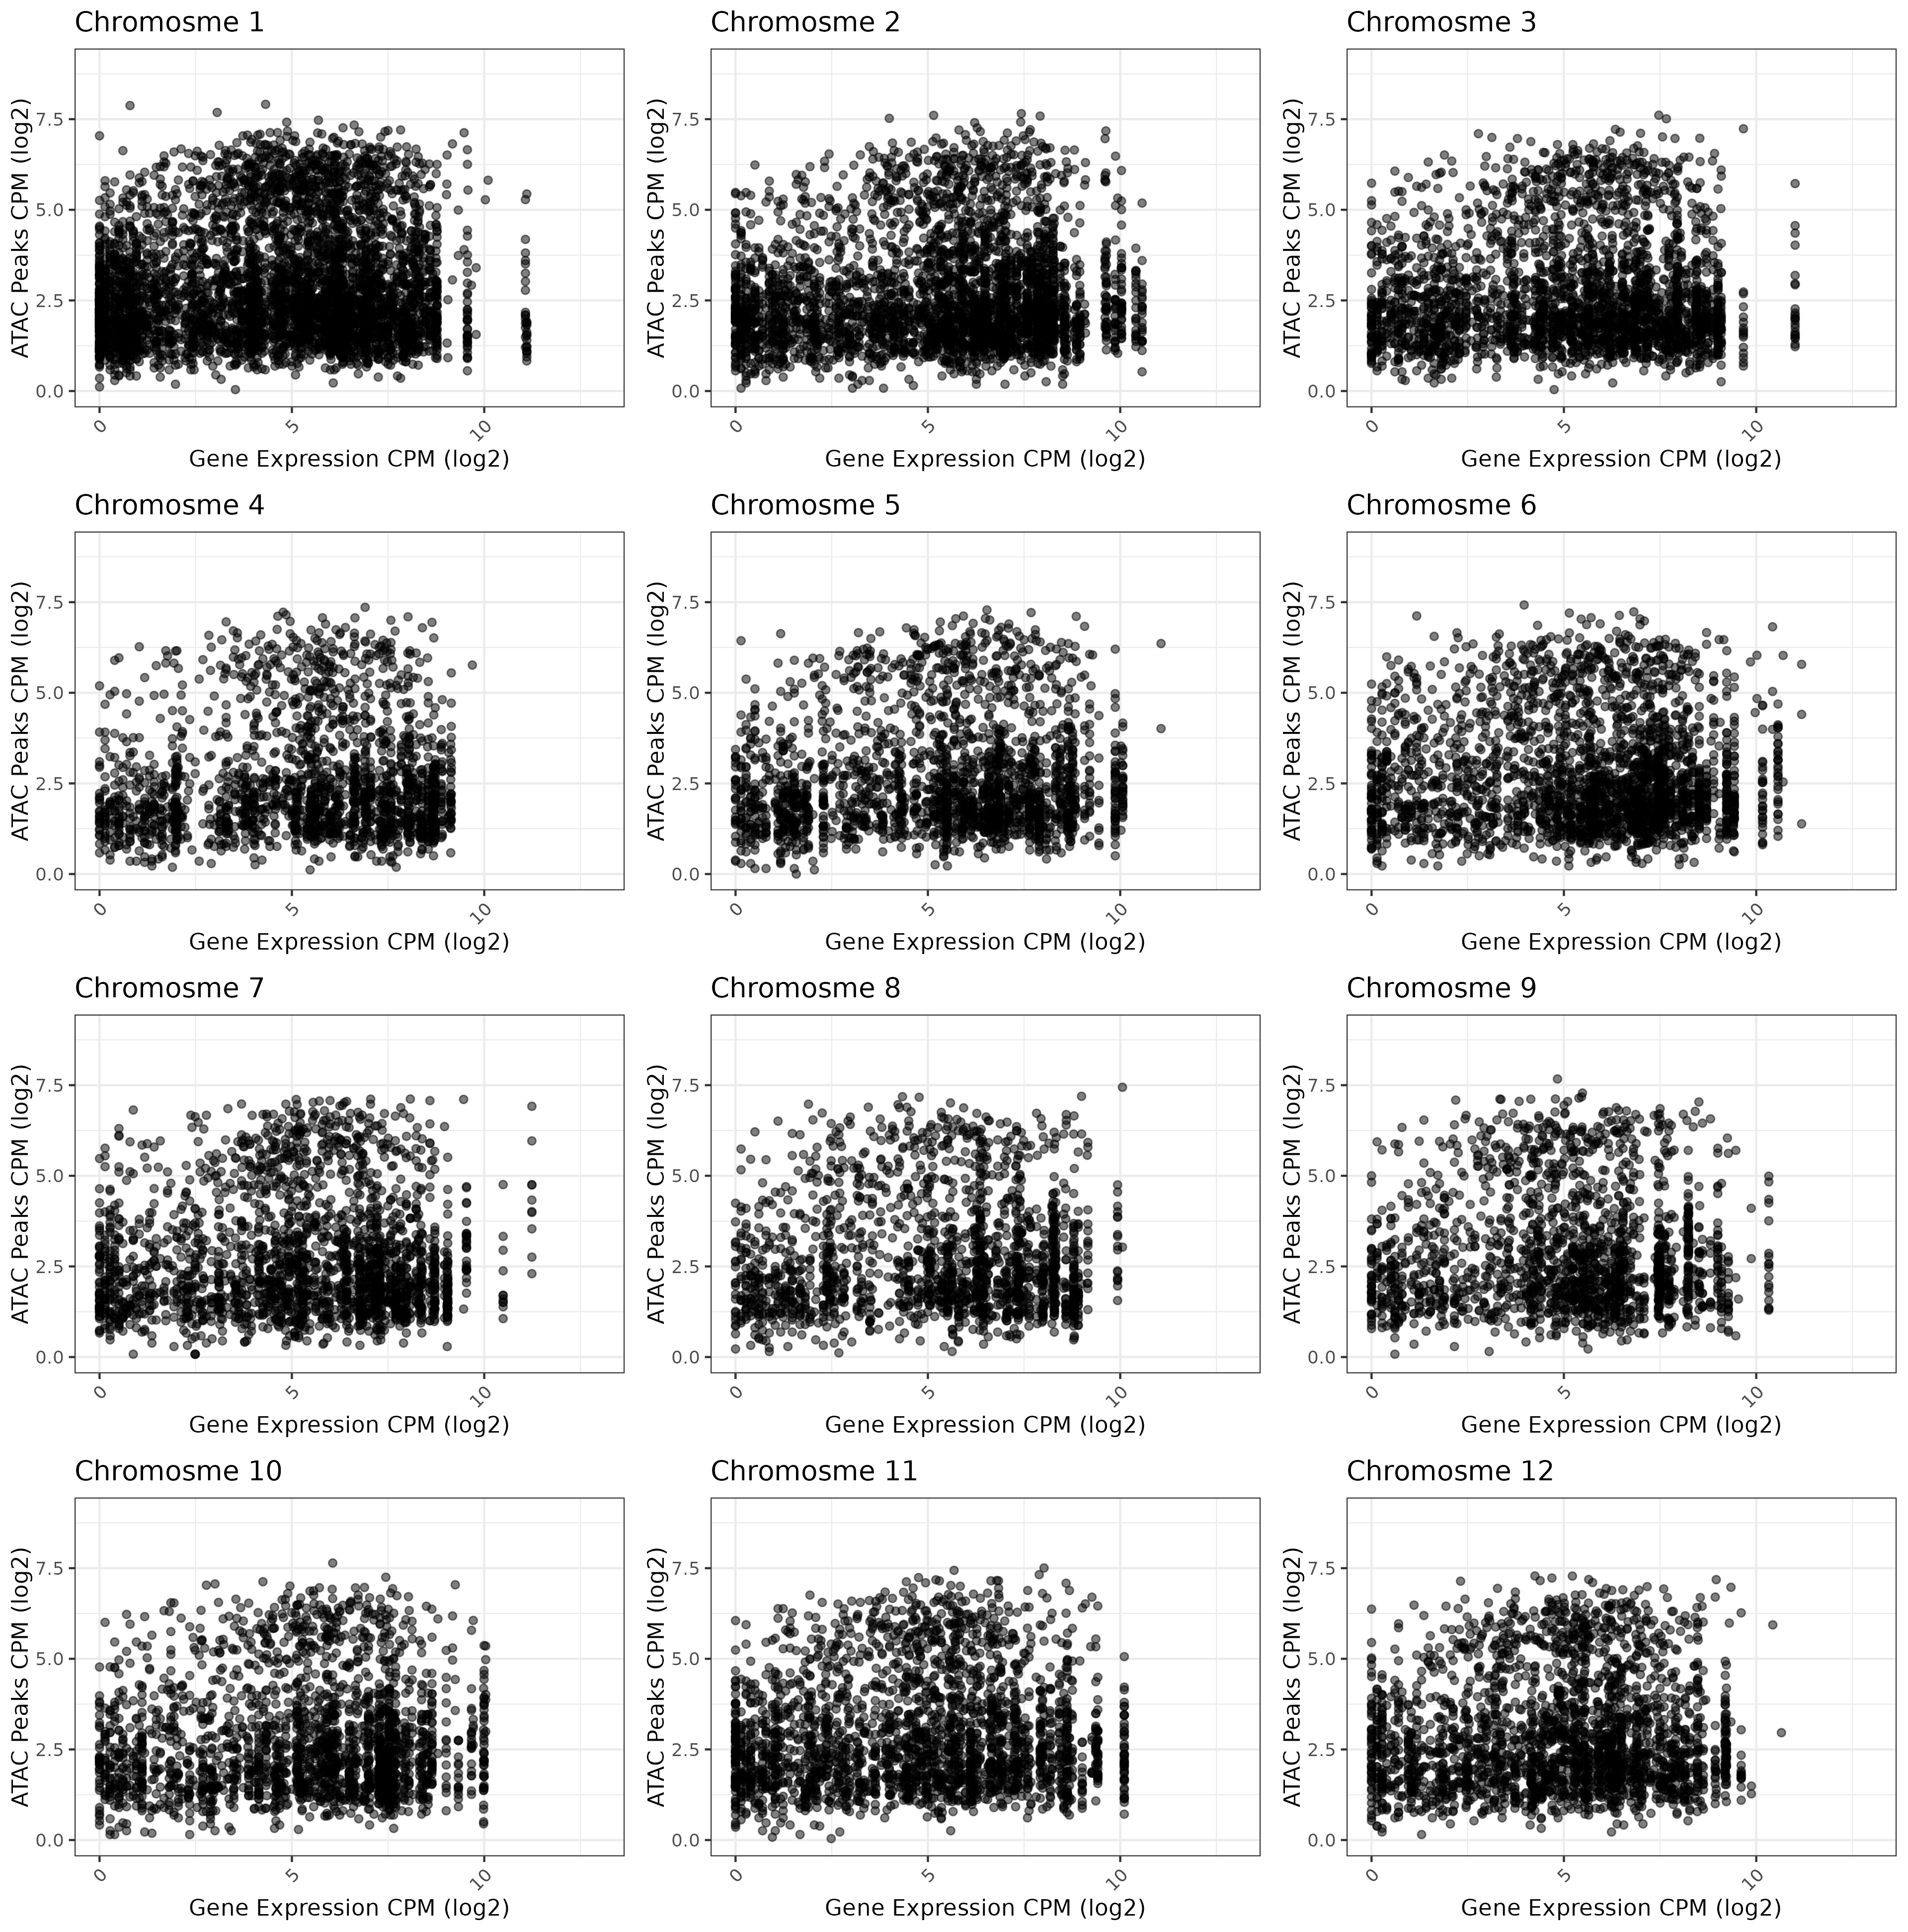
\includegraphics{./Results/s8_plot_1.png}
\caption{Scatter plot for Chromosomes 1 to 12}
\end{figure}

\newpage

\begin{figure}
\centering
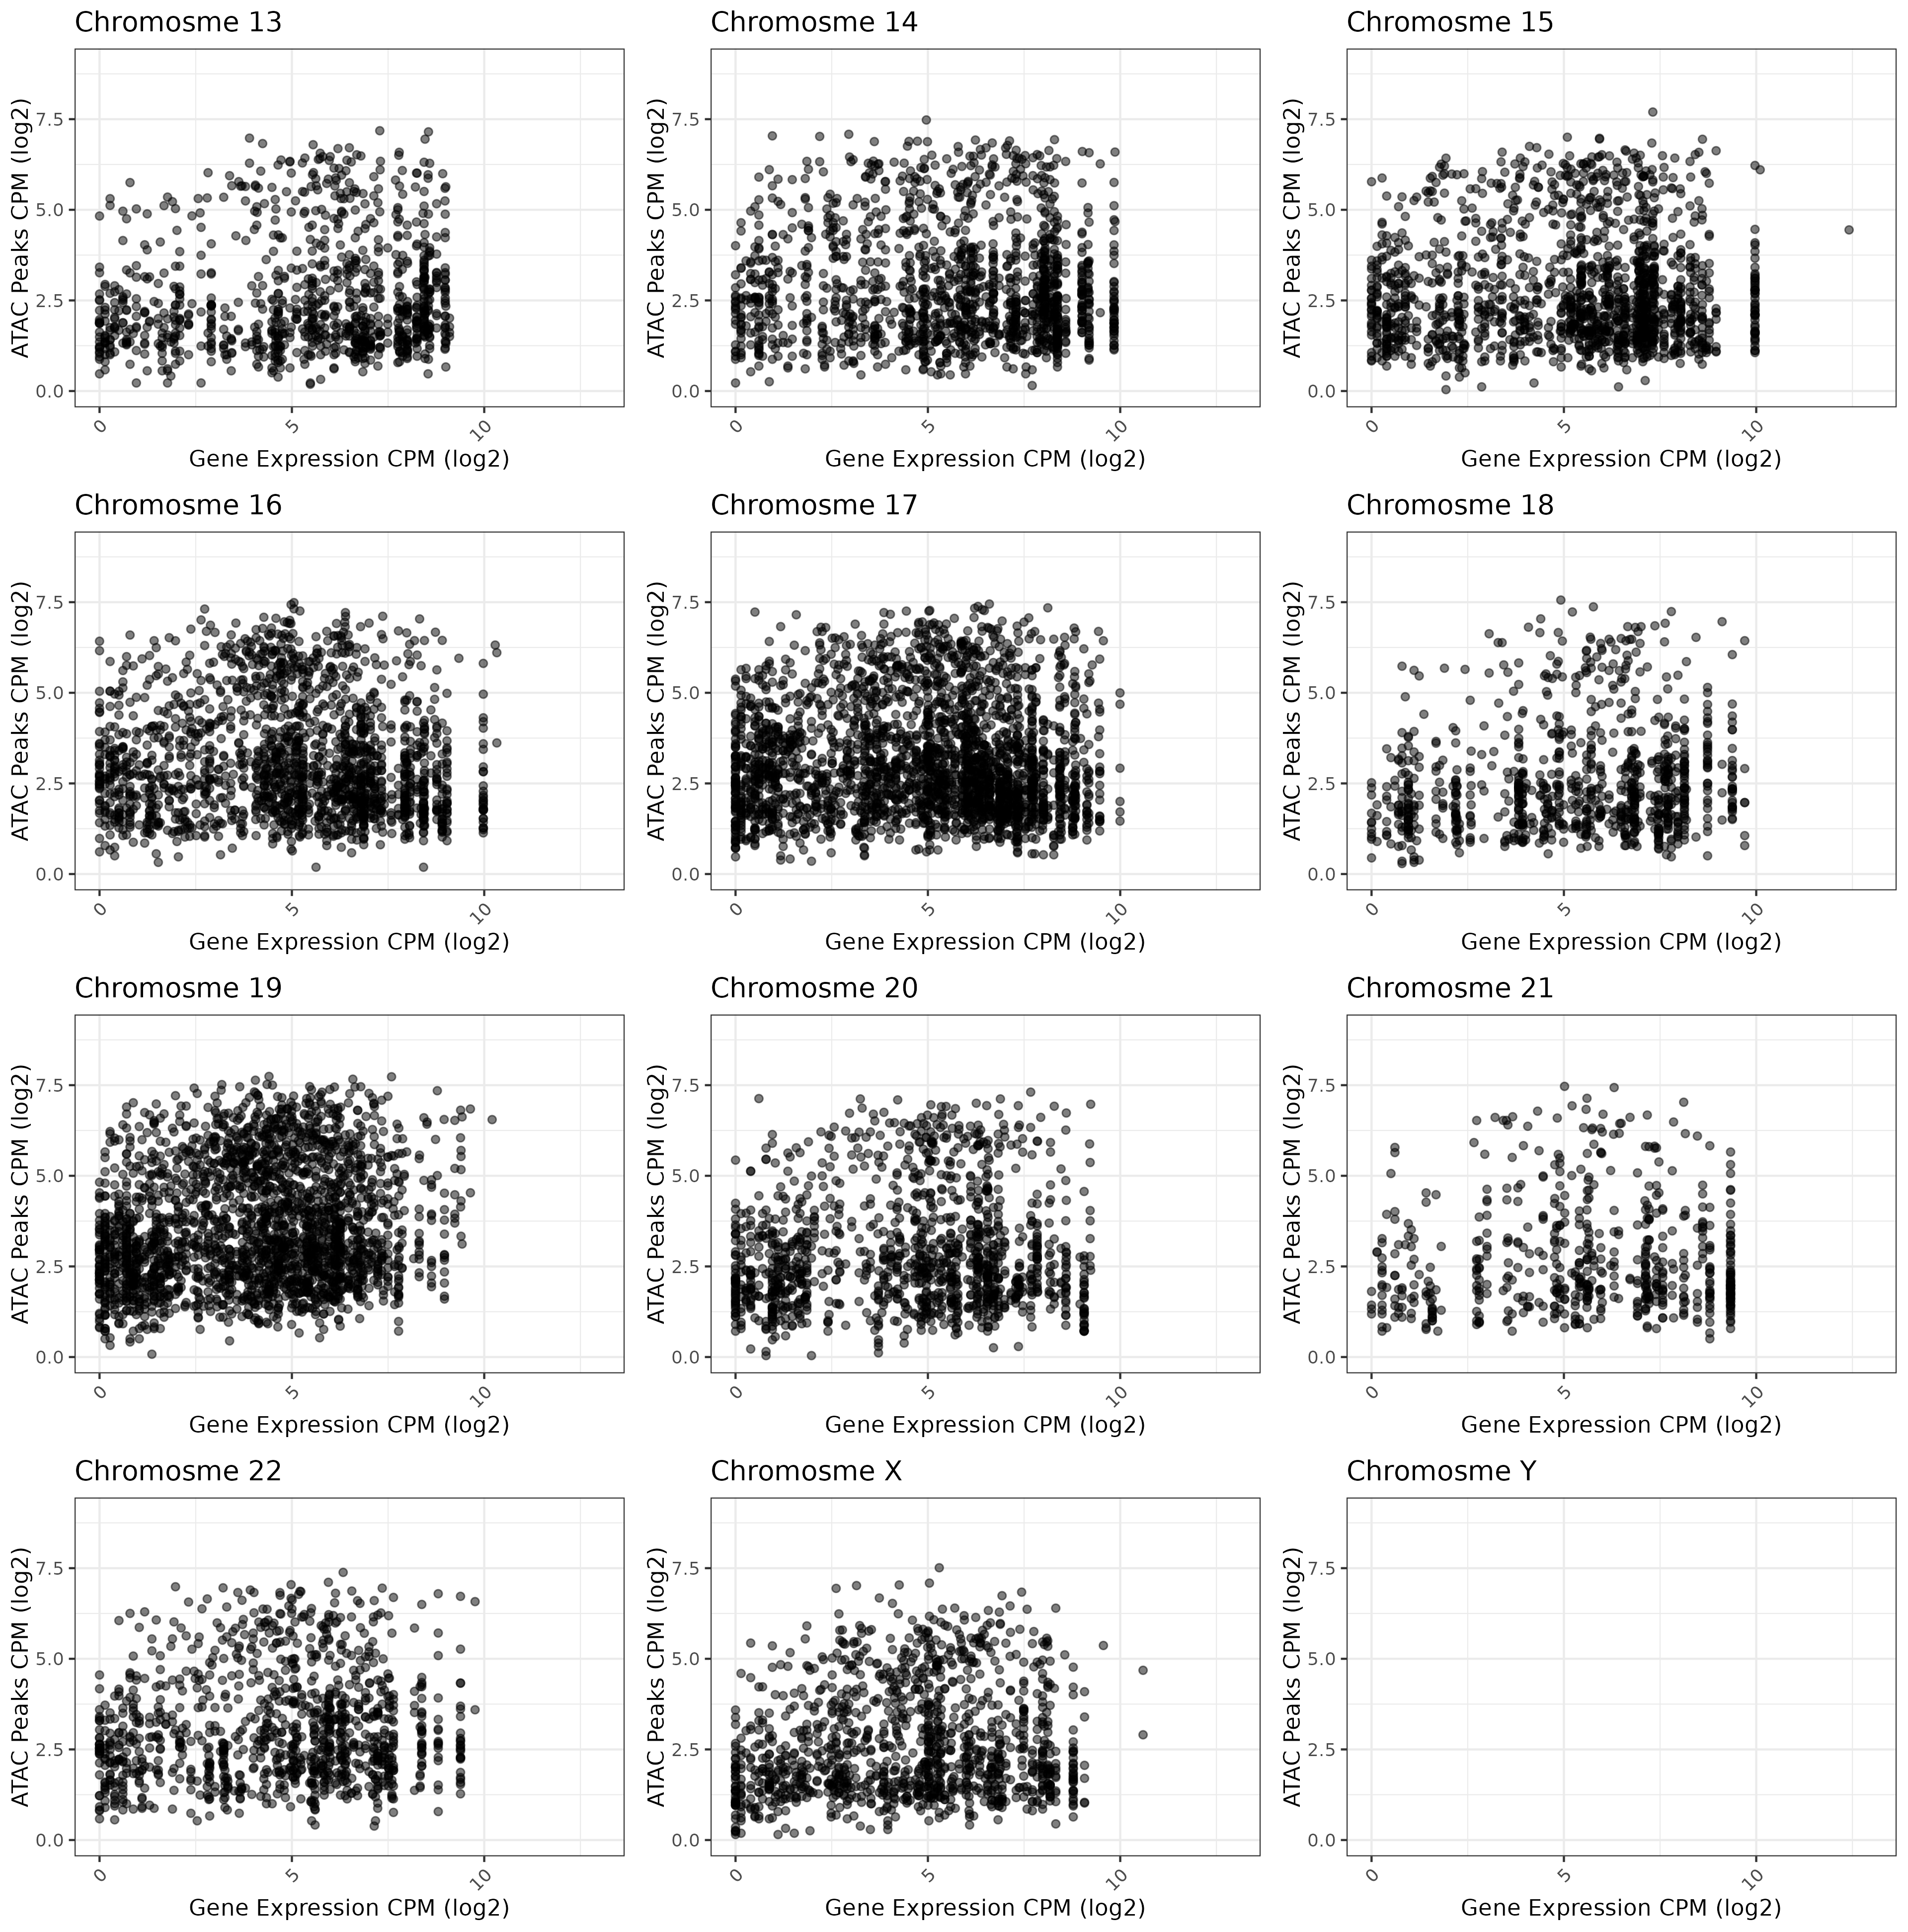
\includegraphics{./Results/s8_plot_2.png}
\caption{Scatter plot for Chromosomes 13 to 22, X, and Y}
\end{figure}

\newpage

\hypertarget{part-4-generation-of-the-r-markdown-file}{%
\section{Part 4: Generation of the R Markdown
file}\label{part-4-generation-of-the-r-markdown-file}}

\begin{Shaded}
\begin{Highlighting}[]
\NormalTok{rmarkdown}\OperatorTok{::}\KeywordTok{render}\NormalTok{(}\StringTok{"Maiolino_Au.Rmd"}\NormalTok{)}
\end{Highlighting}
\end{Shaded}

\end{document}
